\tikzset{every picture/.style={line width=0.75pt}}
\begin{tikzpicture}[x=0.75pt,y=0.75pt,yscale=-1,xscale=1]
	\node (image) {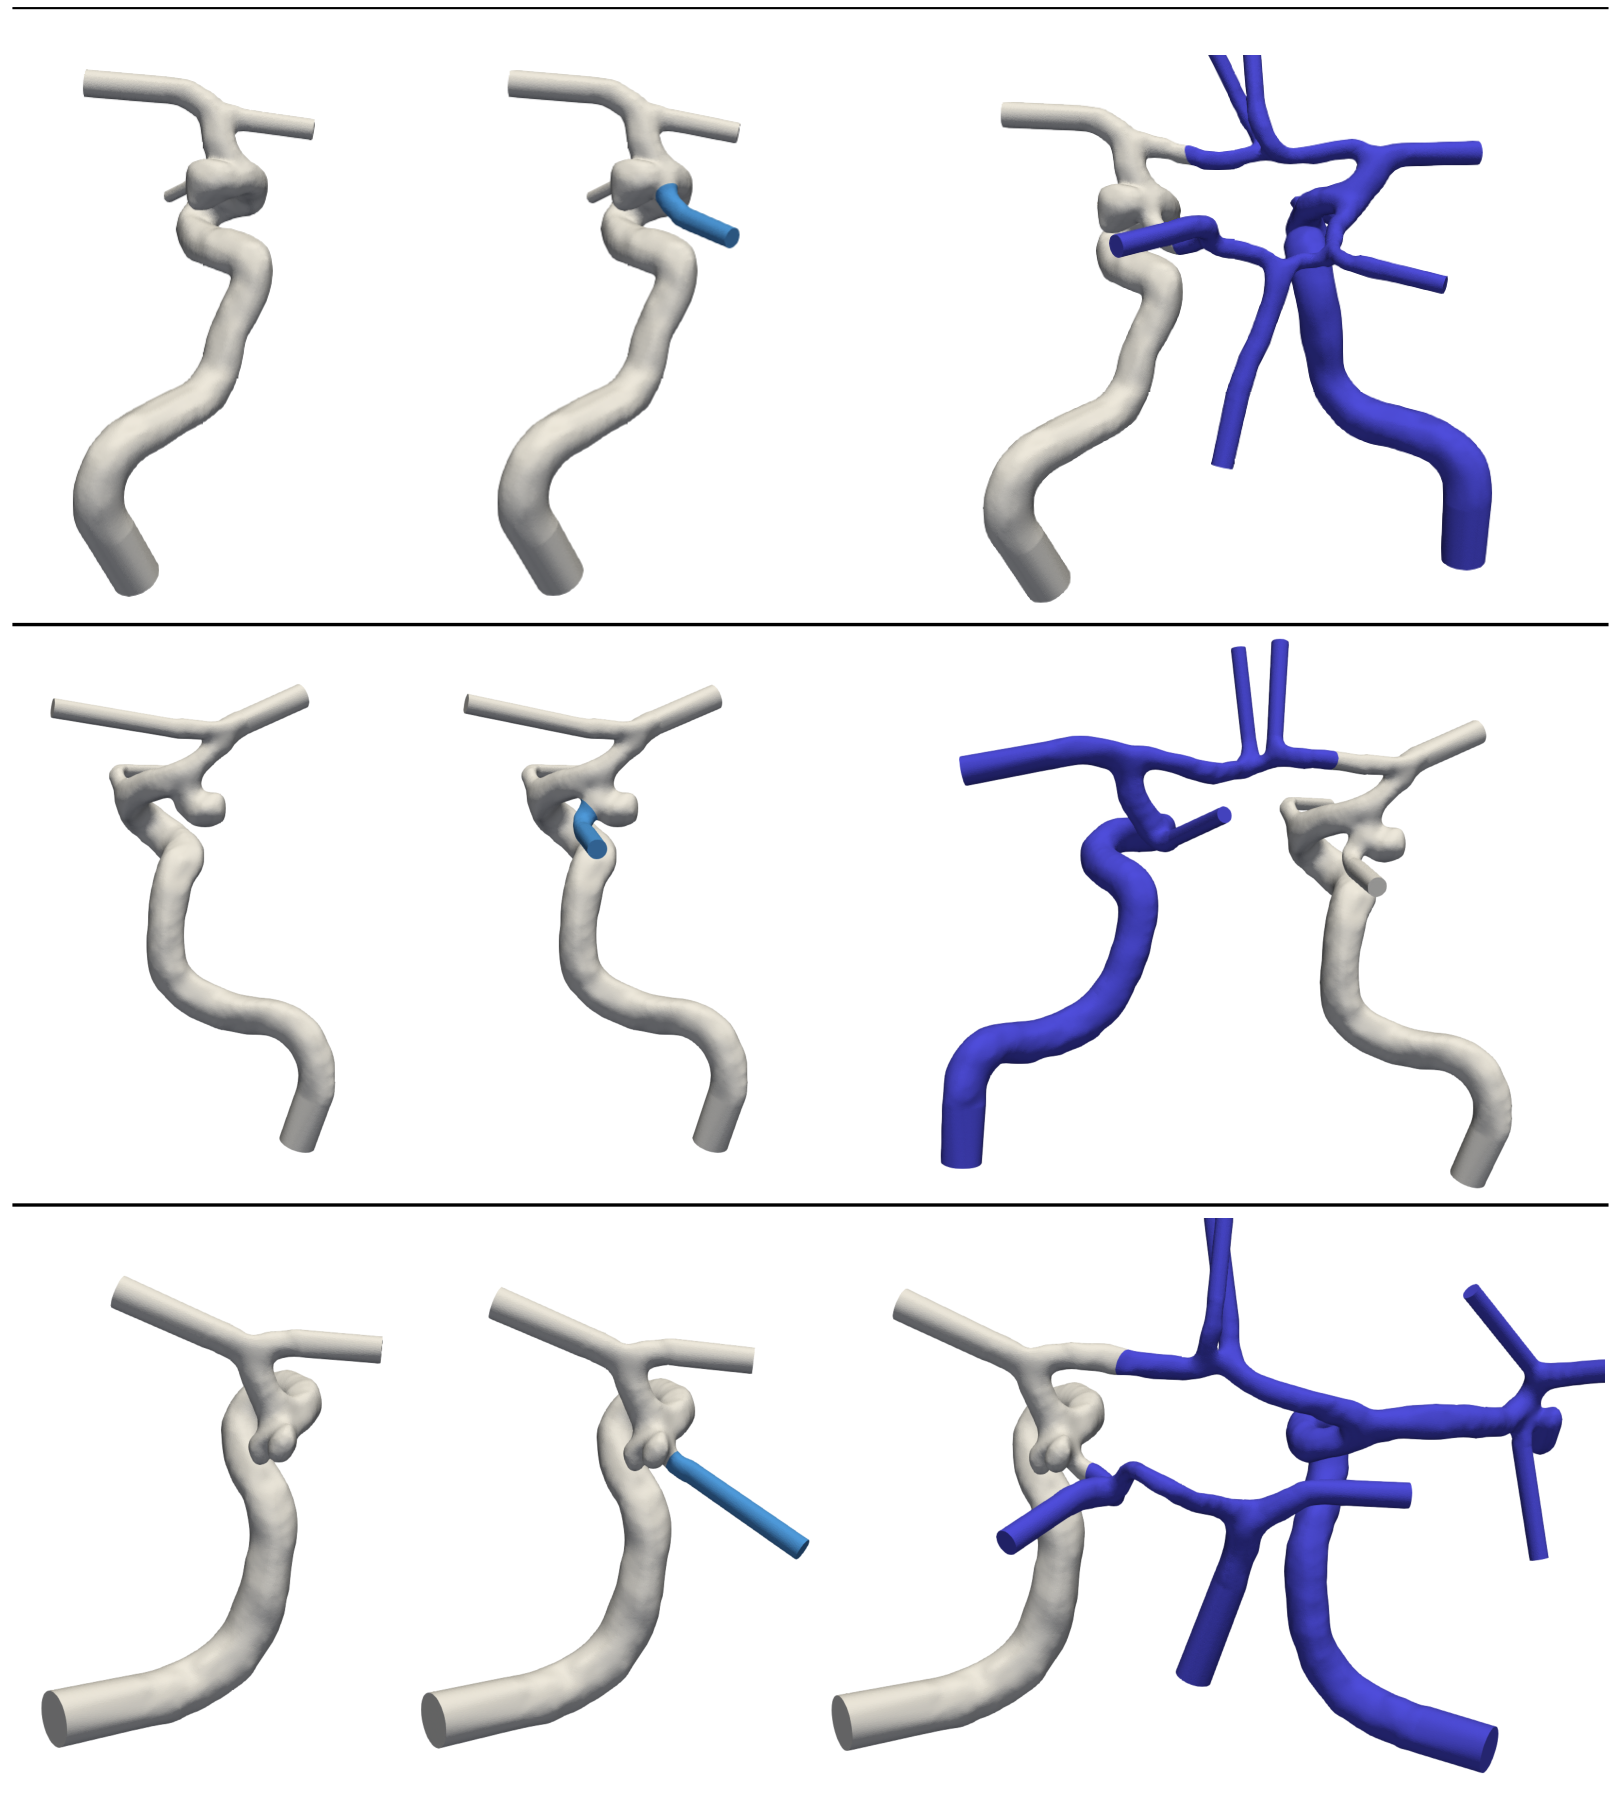
\includegraphics[width=0.8\linewidth]{chapter3/Figures/Study/overview.png}};
	\node[rotate=-270, anchor=center, align=left] at ([xshift=-10pt, yshift=-125pt]image.west) {\textit{Patient A}};
	\node[rotate=-270, anchor=center, align=left] at ([xshift=-10pt]image.west) {\textit{Patient B}};
	\node[rotate=-270, anchor=center, align=left] at ([xshift=-10pt, yshift=125pt]image.west) {\textit{Patient C}};
	\node[anchor=center, align=left] at ([xshift=45pt, yshift=-10pt]image.north west) {\textit{Simplified}};
	\node[anchor=center, align=left] at ([xshift=-35pt, yshift=-10pt]image.north) {\textit{Middle}};
	\node[anchor=center, align=left] at ([xshift=-80pt, yshift=-10pt]image.north east) {\textit{Full}};
\end{tikzpicture}